\documentclass[calcdimensions,landscape,letterpaper]{powersem}
\usepackage{color}
\usepackage[pdftex]{thumbpdf} % For thumbnails
\usepackage[pdftex]{hyperref} % For links.
\usepackage[display,coloremph,whitebackground]{texpower} % colormath
\usepackage{fixseminar}
\usepackage{tpslifonts}
\usepackage[pdftex,final]{graphicx} % For including graphics.
\usepackage{animate}
\usepackage[utf8]{inputenc}
\usepackage{minted}
\usepackage{amsmath}
\usepackage{amssymb}
\usepackage{eurosym}
\usepackage{booktabs} % rules in tables
\usepackage{multirow} % multi-row cells
\usepackage{rotating} % text rotation

\title{A Short Introduction to OpenGL}
\author{Jan Wedekind}
\date{Thursday, May 30th 2024}

\DeclareGraphicsExtensions{.jpg,.pdf,.png}
\pdfcompresslevel=9

\hypersetup{
   pdftitle          = {\thetitle},
   pdfsubject        = {Short OpenGL Presentation 30th May 2024},
   pdfauthor         = {Jan Wedekind},
   pdfkeywords       = {opengl, graphics, software},
   pdfcreator        = {okular},
   pdfproducer       = {LaTeX with TexPower and Minted},
   bookmarksopen     = false,
   bookmarksnumbered = true,
   colorlinks        = true
}

\DeclarePanel{top}{
  \begin{picture}(0,0)
    \put(-3, -293){\resizebox*{\pdfpagewidth}{\pdfpageheight}{
\includegraphics{slide.png}}}
    \put(-10,-20){\parbox[c]{.9\textwidth}{\center\large\bf\thecurrentheading}}
  \end{picture}
}

\DeclarePanel{bottom}{
  \begin{picture}(0,0)
    \put(0,15){\parbox[c]{.98\pdfpagewidth}{\tiny\thedate\hfill\theslide/53}}
  \end{picture}
}

\slidesmag{4}
\backgroundstyle{none}
\slideframe{none}
\pagestyle{empty}

\mklength{\slideleftmargin}{-2cm}
\mklength{\sliderightmargin}{-2cm}
\mklength{\slidetopmargin}{2.0cm}
\mklength{\slidebottommargin}{1.5cm}

\renewcommand{\currentpagevalue}{\value{slide}}
\newcommand{\thecurrentheading}{}
\newcommand{\heading}[1]{\renewcommand{\thecurrentheading}{#1}}
\newcommand{\subheading}[1]{\concept{#1}}

\begin{document}

\begin{slide}
  \pdfbookmark[1]{\thetitle}{title}
  \heading{\ }
  \begin{center}
    \maketitle
  \end{center}
\end{slide}

\begin{slide}
  \pdfbookmark[1]{Motivation}{motivation}
  \heading{Motivation}
  \begin{center}
    \resizebox*{.5\textwidth}{!}{
\includegraphics{logo}}\bigskip\\
    \begin{minipage}[c]{\textwidth}
      \begin{itemize}
          \item cross-platform
          \item less verbose than Vulkan, but knowledge transferable to Vulkan
          \item bindings for many languages
      \end{itemize}
    \end{minipage}
  \end{center}
\end{slide}

\begin{slide}
  \pdfbookmark[1]{Showcase}{showcase}
  \heading{Showcase}
  \begin{center}
    \begin{minipage}[c]{.47\textwidth}
      \begin{center}
        \resizebox*{\textwidth}{!}{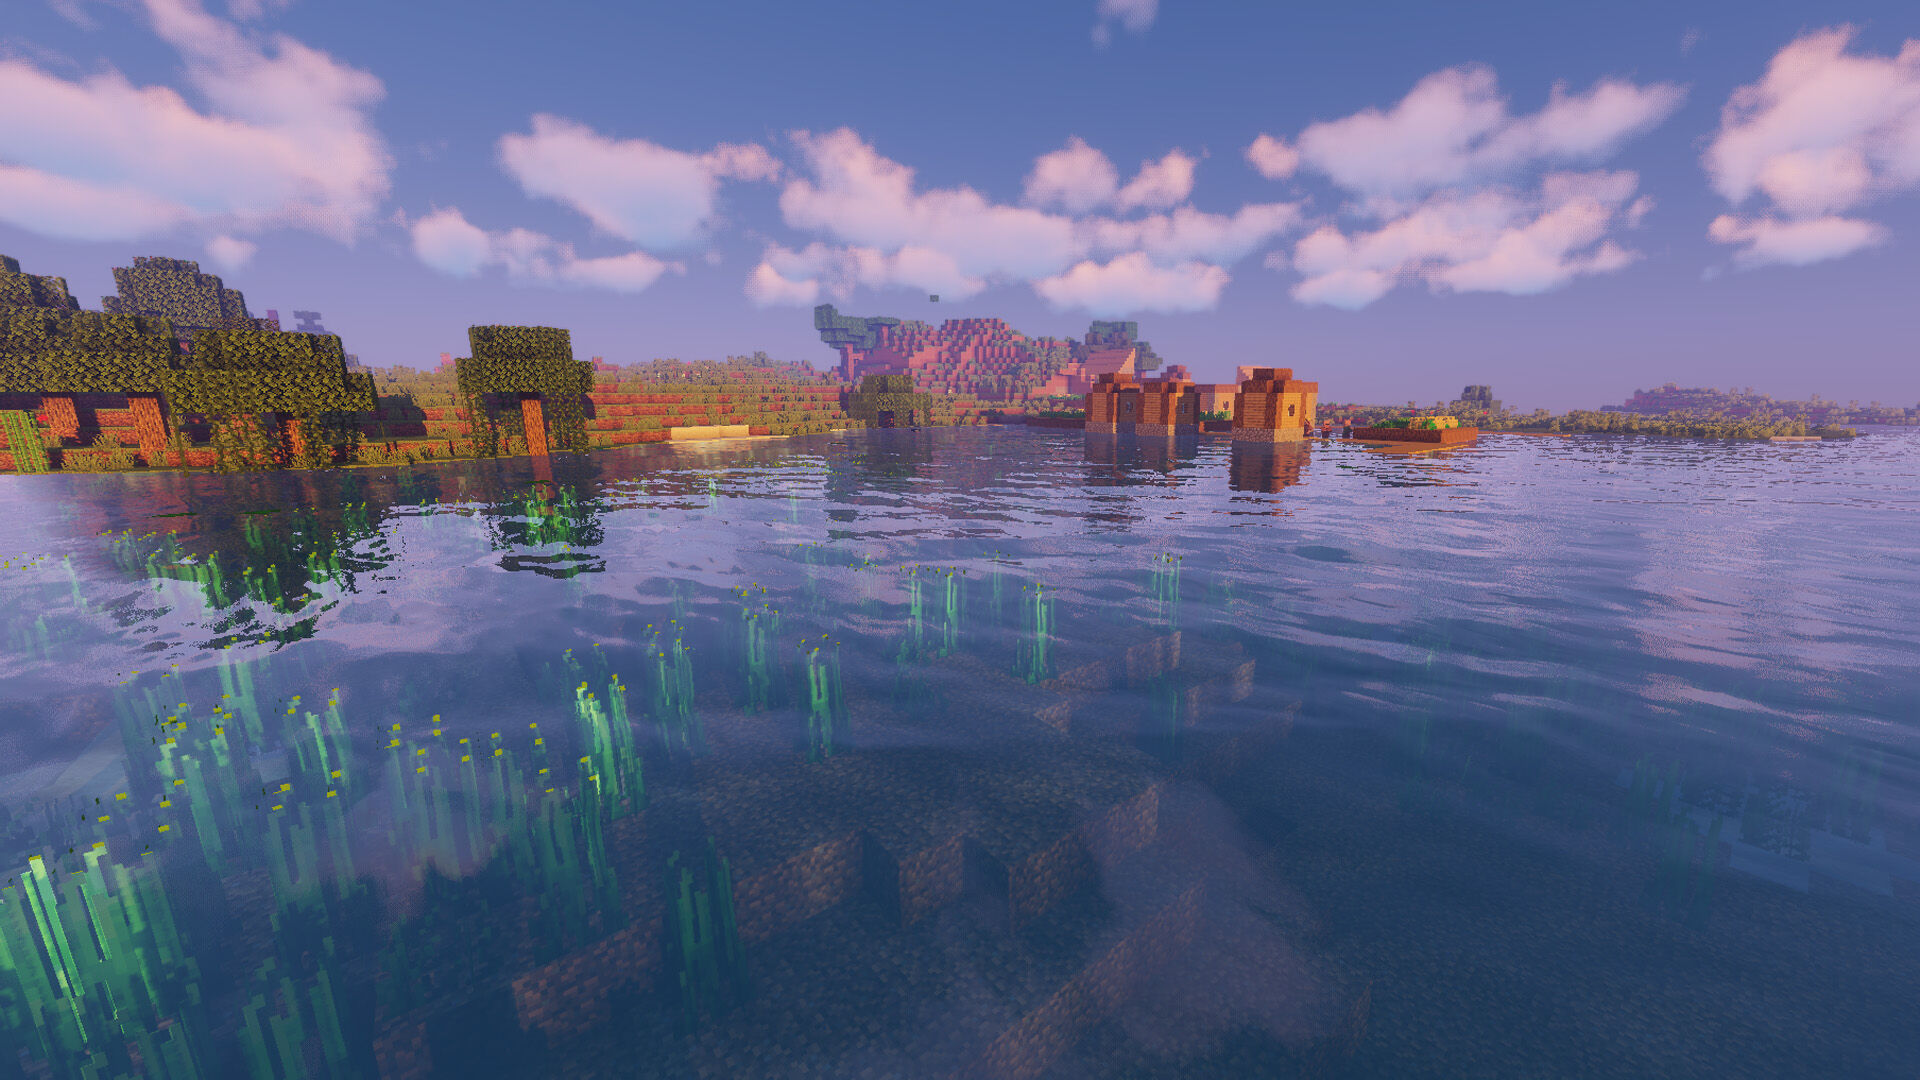
\includegraphics{minecraft}}\\
        Minecraft Java Edition
      \end{center}
    \end{minipage}
    \begin{minipage}[c]{.47\textwidth}
      \begin{center}
        \resizebox*{\textwidth}{!}{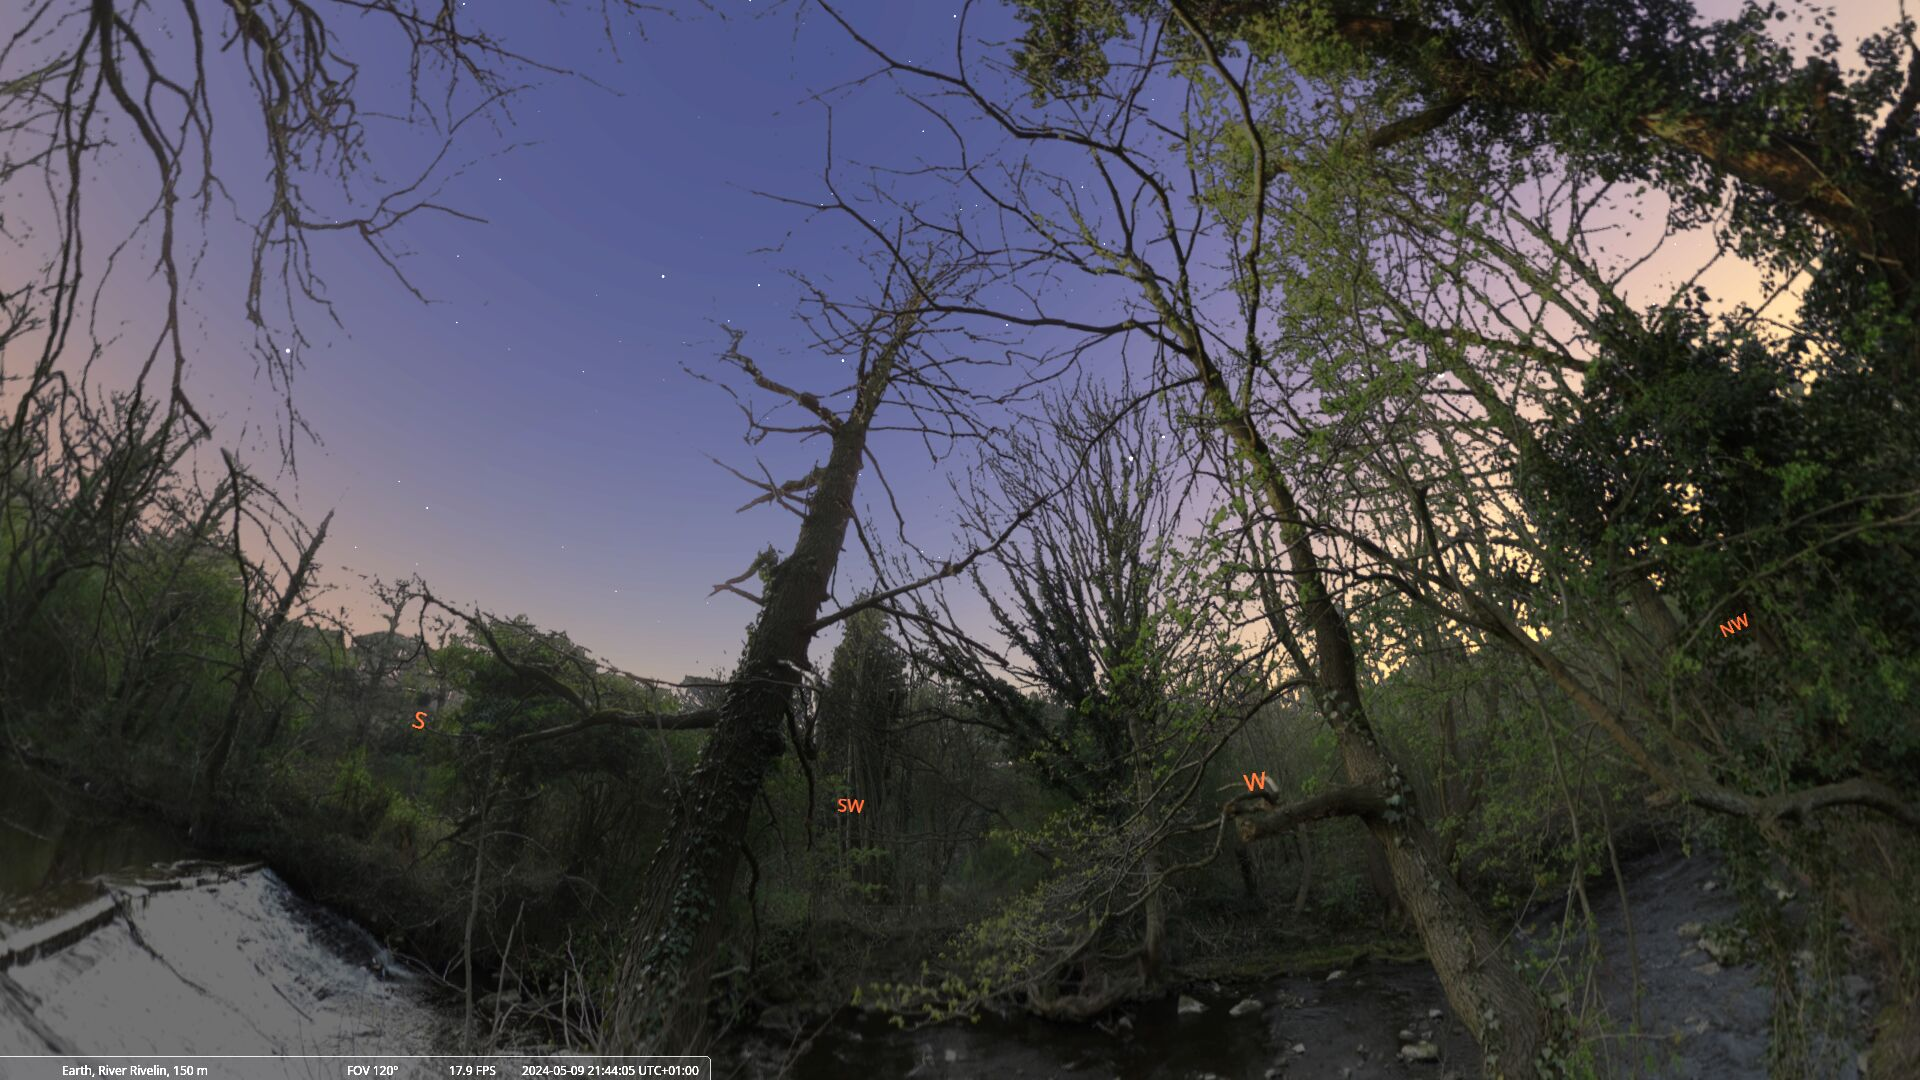
\includegraphics{stellarium}}\\
        Stellarium
      \end{center}
    \end{minipage}\bigskip\\
    \begin{minipage}[c]{.47\textwidth}
      \begin{center}
        \resizebox*{\textwidth}{!}{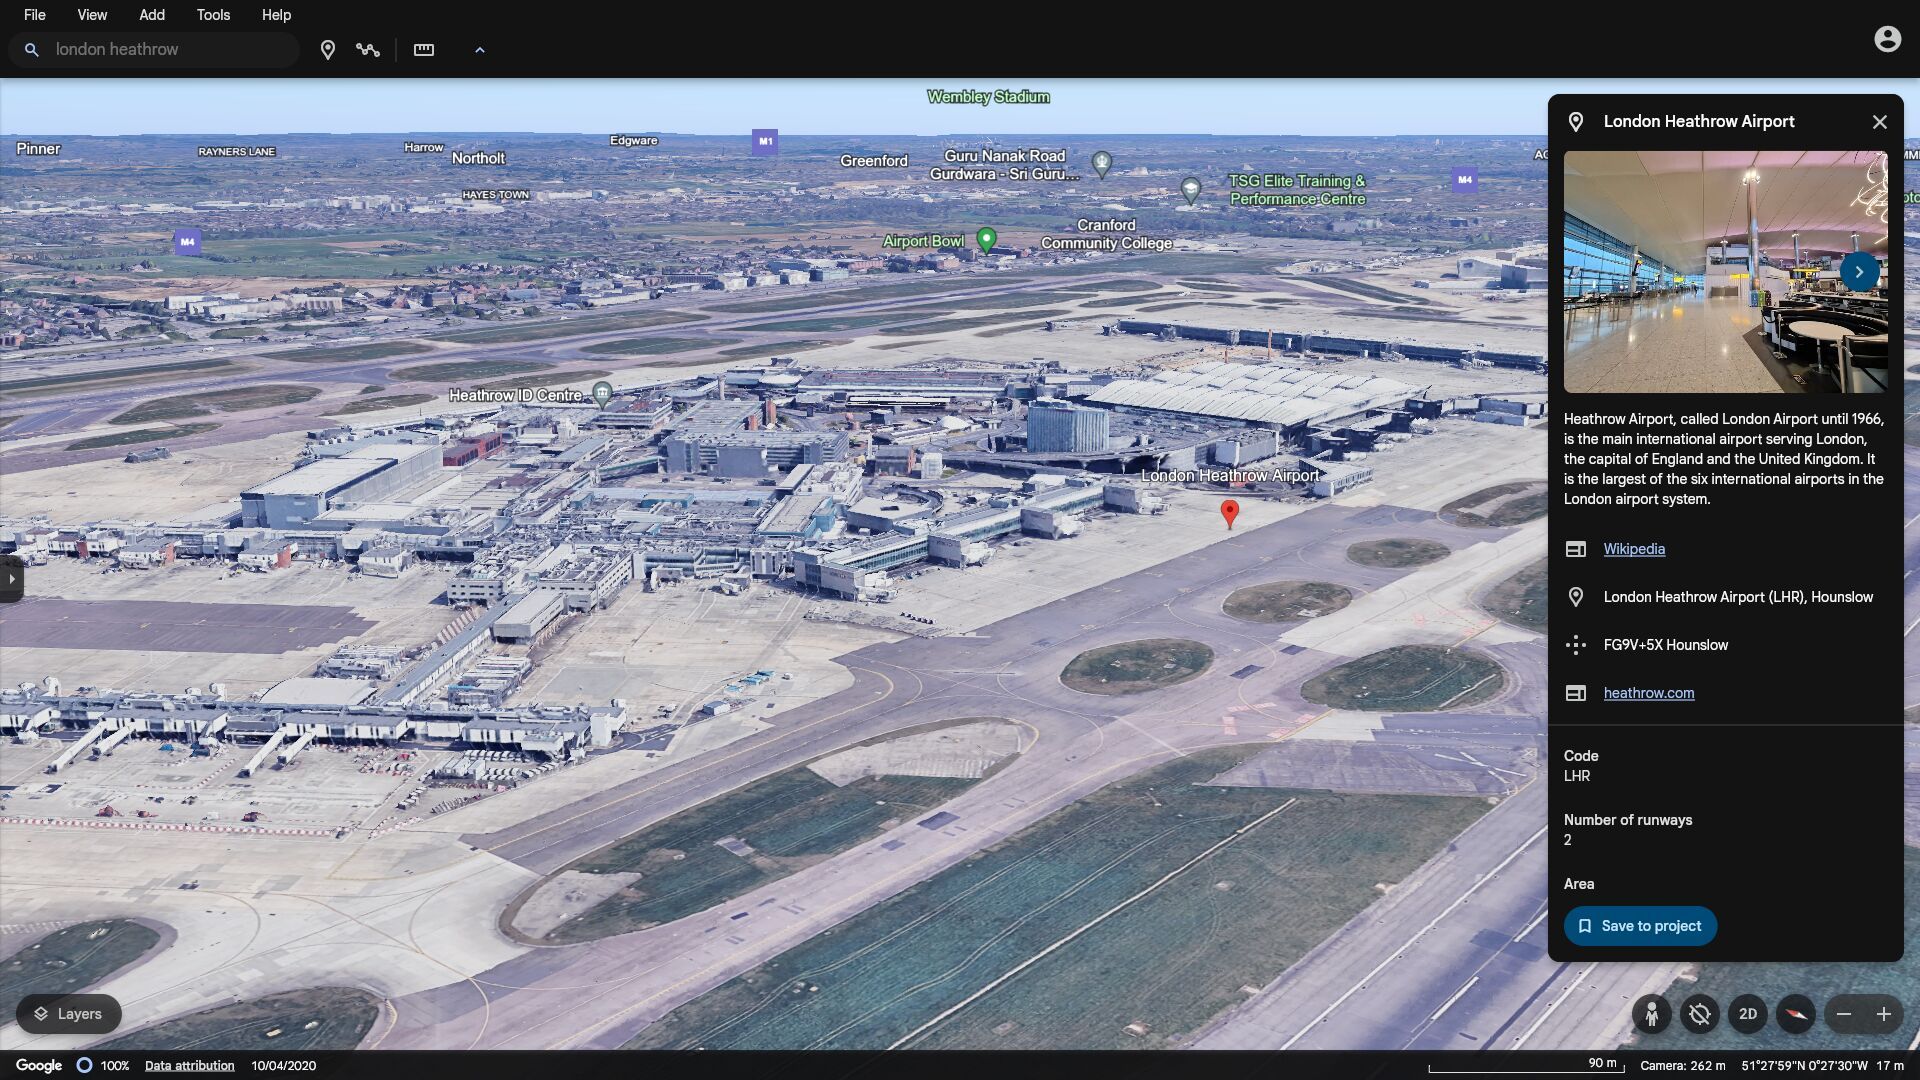
\includegraphics{google-earth}}\\
        WebGL (e.g. Google Earth)
      \end{center}
    \end{minipage}
    \begin{minipage}[c]{.47\textwidth}
      \begin{center}
        \resizebox*{\textwidth}{!}{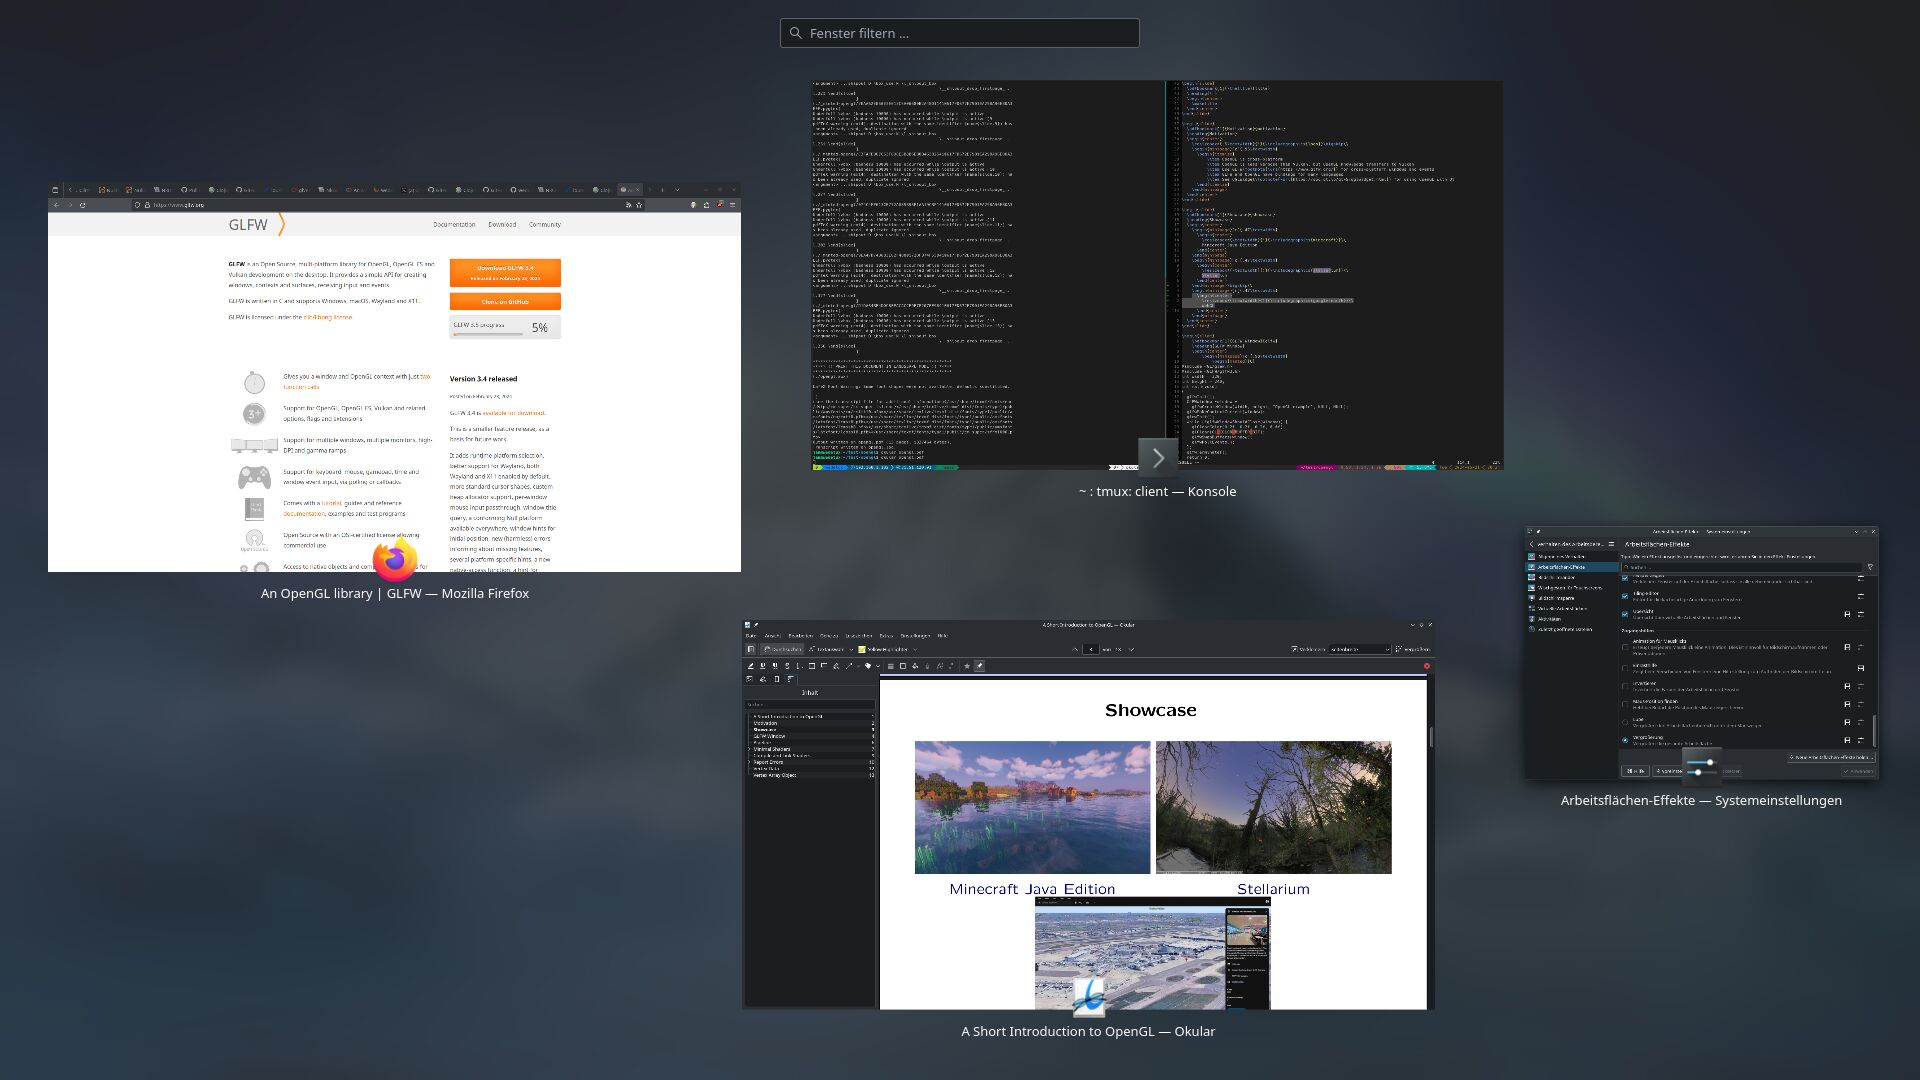
\includegraphics{kde}}\\
        KDE Plasma desktop
      \end{center}
    \end{minipage}
  \end{center}
\end{slide}

\begin{slide}
    \pdfbookmark[2]{GLEW and GLFW}{glew-and-glfw}
    \heading{Getting Started: GLEW and GLFW}
    \begin{center}
        \begin{minipage}[c]{.8\textwidth}
            OpenGL interface and window management
            \begin{itemize}
                \item OpenGL Extension Wrangler Library (GLEW\footnote{\url{https://glew.sourceforge.net/}})
                \item Graphics Library Framework (GLFW\footnote{\url{https://www.glfw.org/}})
            \end{itemize}
        \end{minipage}
    \end{center}
\end{slide}

\begin{slide}
  \pdfbookmark[1]{Getting Started}{getting-started}
    \pdfbookmark[2]{GLFW Window}{glfw}
    \heading{Getting Started: GLFW Window}
    \begin{center}
        \begin{minipage}[c]{.98\textwidth}
            \begin{minted}[highlightlines={11,14}]{C}
#include <GL/glew.h>
#include <GLFW/glfw3.h>
int width = 320; int height = 240;
void main(void)
{
  glfwInit();
  GLFWwindow *window =
    glfwCreateWindow(width, height, "OpenGL example", NULL, NULL);
  glfwMakeContextCurrent(window);
  glewInit();
  glClearColor(0.2f, 0.2f, 0.2f, 0.0f);
  glViewport(0, 0, width, height);
  while (!glfwWindowShouldClose(window)) {
    glClear(GL_COLOR_BUFFER_BIT);
    glfwSwapBuffers(window); glfwPollEvents();
  };
  glfwTerminate();
}
            \end{minted}
        \end{minipage}
    \end{center}
\end{slide}

\begin{slide}
    \pdfbookmark[2]{Result}{glfw-result}
    \heading{Getting Started: Result}
    \begin{center}
      \resizebox*{.9\textwidth}{!}{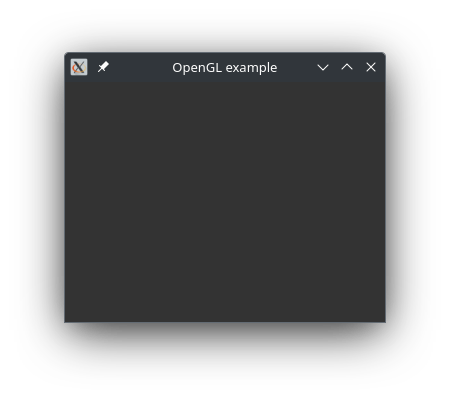
\includegraphics{glfw-window}}
    \end{center}
\end{slide}

\begin{slide}
  \pdfbookmark[1]{Minimal Pipeline}{minimal-pipeline}
  \pdfbookmark[2]{Overview}{minimal-overview}
  \heading{Minimal Pipeline: Overview}
  \begin{center}
    \resizebox*{.6\textwidth}{!}{
\includegraphics{pipeline-minimal}}
  \end{center}
\end{slide}

\begin{slide}
    \pdfbookmark[2]{Shader Code}{minimal-glsl}
    \heading{Minimal Pipeline: Shader Code (GLSL)}
    \begin{center}
        \begin{minipage}[c]{.5\textwidth}
            \begin{minted}[highlightlines={5}]{glsl}
#version 410 core
in vec3 point;
void main()
{
  gl_Position = vec4(point, 1);
}
            \end{minted}
            \vspace{-10pt}
            \rule{4cm}{0.4pt}
            \begin{minted}[highlightlines={5}]{glsl}
#version 410 core
out vec3 fragColor;
void main()
{
  fragColor = vec3(1, 0, 0);
}
            \end{minted}
        \end{minipage}
    \end{center}
\end{slide}

\begin{slide}
    \pdfbookmark[2]{C Strings}{c-strings}
    \heading{Minimal Pipeline: C Strings}
    \begin{center}
        \begin{minipage}[c]{.7\textwidth}
            \begin{minted}{C}
const char *vertexSource = "#version 410 core\n\
in vec3 point;\n\
void main()\n\
{\n\
  gl_Position = vec4(point, 1);\n\
}";

const char *fragmentSource = "#version 410 core\n\
out vec3 fragColor;\n\
void main()\n\
{\n\
  fragColor = vec3(1, 0, 0);\n\
}";
            \end{minted}
        \end{minipage}
    \end{center}
\end{slide}

\begin{slide}
    \pdfbookmark[2]{Compile and Link Shaders}{compile-minimal}
    \heading{Minimal Pipeline: Compile \& Link Shaders}
    \begin{center}
        \begin{minipage}[c]{.95\textwidth}
            \begin{minted}[highlightlines={4,9,13-15}]{C}
  // ...
  GLuint vertexShader = glCreateShader(GL_VERTEX_SHADER);
  glShaderSource(vertexShader, 1, &vertexSource, NULL);
  glCompileShader(vertexShader);
  handleCompileError("Vertex shader", vertexShader);

  GLuint fragmentShader = glCreateShader(GL_FRAGMENT_SHADER);
  glShaderSource(fragmentShader, 1, &fragmentSource, NULL);
  glCompileShader(fragmentShader);
  handleCompileError("Fragment shader", fragmentShader);

  GLuint program = glCreateProgram();
  glAttachShader(program, vertexShader);
  glAttachShader(program, fragmentShader);
  glLinkProgram(program);
  handleLinkError("Shader program", program);
  // ...
            \end{minted}
        \end{minipage}
    \end{center}
\end{slide}

\begin{slide}
    \pdfbookmark[2]{Compile Errors}{compile-error}
    \heading{Minimal Pipeline: Compile Errors}
    \begin{center}
        \begin{minipage}[c]{.95\textwidth}
            \begin{minted}[highlightlines={6,9}]{C}
#include <stdio.h>
// ...
void handleCompileError(const char *step, GLuint shader)
{
  GLint result = GL_FALSE;
  glGetShaderiv(shader, GL_COMPILE_STATUS, &result);
  if (result == GL_FALSE) {
    char buffer[1024];
    glGetShaderInfoLog(shader, 1024, NULL, buffer);
    if (buffer[0]) fprintf(stderr, "%s: %s\n", step, buffer);
  };
}
// ...
            \end{minted}
        \end{minipage}
    \end{center}
\end{slide}

\begin{slide}
    \pdfbookmark[2]{Link Errors}{link-error}
    \heading{Minimal Pipeline: Link Errors}
    \begin{center}
        \begin{minipage}[c]{.95\textwidth}
            \begin{minted}[highlightlines={6,9}]{C}
#include <stdio.h>
// ...
void handleLinkError(const char *step, GLuint program)
{
  GLint result = GL_FALSE;
  glGetProgramiv(program, GL_LINK_STATUS, &result);
  if (result == GL_FALSE) {
    char buffer[1024];
    glGetProgramInfoLog(program, 1024, NULL, buffer);
    if (buffer[0]) fprintf(stderr, "%s: %s\n", step, buffer);
  };
}
// ...
            \end{minted}
        \end{minipage}
    \end{center}
\end{slide}

\begin{slide}
    \pdfbookmark[1]{Pipeline Input}{pipeline-input}
    \pdfbookmark[2]{Vertex and Index Data}{vertex-index}
    \heading{Pipeline Input: Vertex and Index Data}
    \begin{center}
        \begin{minipage}[b]{.55\textwidth}
            \begin{minted}{C}
// ...
GLfloat vertices[] = {
  //  x,     y,     z
  -0.5f, -0.5f,  0.0f,
   0.5f, -0.5f,  0.0f,
  -0.5f,  0.5f,  0.0f,
   0.5f,  0.5f,  0.0f
};

unsigned int indices[] = {0, 1, 3, 2};

GLuint vao;
GLuint vbo;
GLuint idx;
// ...
            \end{minted}
        \end{minipage}
        \begin{minipage}[b]{.4\textwidth}
          \resizebox*{.9\textwidth}{!}{
\includegraphics{ndc}}\\
          normalised device coordinates (NDC)
        \end{minipage}
    \end{center}
\end{slide}

\begin{slide}
    \pdfbookmark[2]{Vertex Array Object}{vao-data}
    \heading{Pipeline Input: Vertex Array Object}
    \begin{center}
        \begin{minipage}[c]{.95\textwidth}
            \begin{minted}[highlightlines={6-7,10-11,13-15}]{C}
  glGenVertexArrays(1, &vao);
  glBindVertexArray(vao);

  glGenBuffers(1, &vbo);
  glBindBuffer(GL_ARRAY_BUFFER, vbo);
  glBufferData(GL_ARRAY_BUFFER, sizeof(vertices), vertices,
               GL_STATIC_DRAW);
  glGenBuffers(1, &idx);
  glBindBuffer(GL_ELEMENT_ARRAY_BUFFER, idx);
  glBufferData(GL_ELEMENT_ARRAY_BUFFER, sizeof(indices), indices,
               GL_STATIC_DRAW);

  glVertexAttribPointer(glGetAttribLocation(program, "point"),
                        3, GL_FLOAT, GL_FALSE,
                        3 * sizeof(float), (void *)0);

  glUseProgram(program);
  glEnableVertexAttribArray(0);
            \end{minted}
        \end{minipage}
    \end{center}
\end{slide}

\begin{slide}
    \pdfbookmark[2]{Render Quads}{render-quads}
    \heading{Pipeline Input: Render Quads}
    \begin{center}
        \begin{minipage}[c]{.95\textwidth}
            \begin{minted}[highlightlines={4}]{C}
  // ...
  while (!glfwWindowShouldClose(window)) {
    glClear(GL_COLOR_BUFFER_BIT);
    glDrawElements(GL_QUADS, 4, GL_UNSIGNED_INT, (void *)0);
    glfwSwapBuffers(window);
    glfwPollEvents();
  };
  // ...
            \end{minted}
        \end{minipage}
    \end{center}
\end{slide}

\begin{slide}
    \pdfbookmark[2]{Cleanup}{pipeline-clean-up}
    \heading{Pipeline Input: Cleanup}
    \begin{center}
        \begin{minipage}[c]{.7\textwidth}
            \begin{minted}{C}
  // ...
  glDisableVertexAttribArray(0);

  glBindBuffer(GL_ELEMENT_ARRAY_BUFFER, 0);
  glDeleteBuffers(1, &idx);

  glBindBuffer(GL_ARRAY_BUFFER, 0);
  glDeleteBuffers(1, &vbo);

  glBindVertexArray(0);
  glDeleteVertexArrays(1, &vao);

  glDeleteProgram(program);
  glDeleteShader(vertexShader);
  glDeleteShader(fragmentShader);

  glfwTerminate();
  // ...
            \end{minted}
        \end{minipage}
    \end{center}
\end{slide}

\begin{slide}
    \pdfbookmark[2]{Result}{pipeline-result}
    \heading{Pipeline Input: Result}
    \begin{center}
      \resizebox*{.9\textwidth}{!}{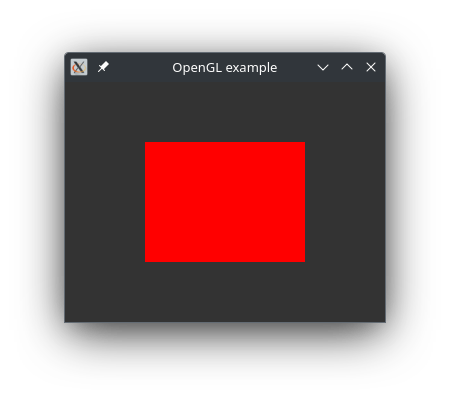
\includegraphics{quad}}
    \end{center}
\end{slide}

\begin{slide}
    \pdfbookmark[1]{Textures}{textures}
    \pdfbookmark[2]{Texture Coordinates and Data}{coords}
    \heading{Textures: Coordinates and Pixels}
    \begin{center}
        \begin{minipage}[c]{.7\textwidth}
            \begin{minted}{C}
// ...
GLfloat vertices[] = {
  //  x,     y,     z,    u,    v
  -0.5f, -0.5f,  0.0f, 0.0f, 0.0f,
   0.5f, -0.5f,  0.0f, 6.0f, 0.0f,
  -0.5f,  0.5f,  0.0f, 0.0f, 6.0f,
   0.5f,  0.5f,  0.0f, 6.0f, 6.0f
};

float chequer[] = {
  // r,    g,    b
  0.4f, 0.4f, 0.4f,
  1.0f, 1.0f, 1.0f,
  1.0f, 1.0f, 1.0f,
  0.4f, 0.4f, 0.4f
};
// ...
            \end{minted}
        \end{minipage}
    \end{center}
\end{slide}

\begin{slide}
    \pdfbookmark[2]{Shaders}{tex-shader}
    \heading{Textures: Shaders}
    \begin{center}
        \begin{minipage}[c]{.5\textwidth}
            \begin{minted}[highlightlines={3,4,8}]{glsl}
#version 410 core
in vec3 point;
in vec2 texcoord;
out vec2 UV;
void main()
{
  gl_Position = vec4(point, 1);
  UV = texcoord;
}
            \end{minted}
            \vspace{-10pt}
            \rule{4cm}{0.4pt}
            \begin{minted}[highlightlines={2,3,7}]{glsl}
#version 410 core
uniform sampler2D tex;
in vec2 UV;
out vec3 fragColor;
void main()
{
  fragColor = texture(tex, UV).rgb;
}
            \end{minted}
        \end{minipage}
    \end{center}
\end{slide}

\begin{slide}
    \pdfbookmark[2]{Multiple Vertex Attributes}{multiple-vertex}
    \heading{Textures: Multiple Vertex Attributes}
    \begin{center}
        \begin{minipage}[c]{.95\textwidth}
            \begin{minted}{C}
  // ...
  glVertexAttribPointer(glGetAttribLocation(program, "point"),
                        3, GL_FLOAT, GL_FALSE,
                        5 * sizeof(float),
                        (void *)0);
  glVertexAttribPointer(glGetAttribLocation(program, "texcoord"),
                        2, GL_FLOAT, GL_FALSE,
                        5 * sizeof(float),
                        (void *)(3 * sizeof(float)));
  glEnableVertexAttribArray(0);
  glEnableVertexAttribArray(1);
  // ...
            \end{minted}
        \end{minipage}
    \end{center}
\end{slide}

\begin{slide}
    \pdfbookmark[2]{Setup}{texture-setup}
    \heading{Textures: Setup}
    \begin{center}
        \begin{minipage}[c]{\textwidth}
            \begin{minted}[highlightlines={4,5,6,7-8}]{C}
  // ...
  GLuint tex;
  glGenTextures(1, &tex);
  glActiveTexture(GL_TEXTURE0 + 0);
  glBindTexture(GL_TEXTURE_2D, tex);
  glUniform1i(glGetUniformLocation(program, "tex"), 0);
  glTexImage2D(GL_TEXTURE_2D, 0, GL_RGB, 2, 2, 0, GL_BGR,
               GL_FLOAT, chequer);
  glTexParameteri(GL_TEXTURE_2D, GL_TEXTURE_WRAP_S, GL_REPEAT);
  glTexParameteri(GL_TEXTURE_2D, GL_TEXTURE_WRAP_T, GL_REPEAT);
  glTexParameteri(GL_TEXTURE_2D, GL_TEXTURE_MIN_FILTER, GL_NEAREST);
  glTexParameteri(GL_TEXTURE_2D, GL_TEXTURE_MAG_FILTER, GL_NEAREST);
  // ...
            \end{minted}
        \end{minipage}
    \end{center}
\end{slide}

\begin{slide}
    \pdfbookmark[2]{Cleanup}{texture-cleanup}
    \heading{Textures: Cleanup}
    \begin{center}
        \begin{minipage}[c]{.6\textwidth}
            \begin{minted}{C}
  // ...
  glBindTexture(GL_TEXTURE_2D, 0);
  glDeleteTextures(1, &tex);
  // ...
            \end{minted}
        \end{minipage}
    \end{center}
\end{slide}

\begin{slide}
    \pdfbookmark[2]{Textures: Result}{texture-quad}
    \heading{Textures: Result}
    \begin{center}
      \resizebox*{.9\textwidth}{!}{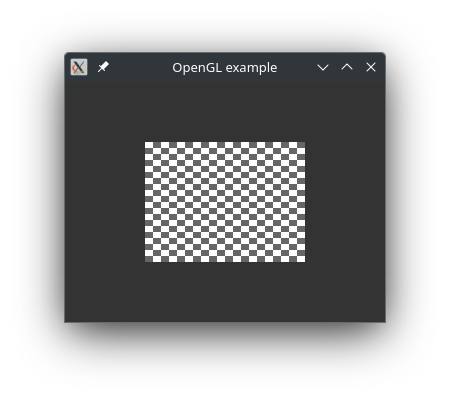
\includegraphics{chequer}}
    \end{center}
\end{slide}

\begin{slide}
    \pdfbookmark[1]{3D}{3d}
    \pdfbookmark[2]{3D: Rotations}{rotation}
    \heading{3D: Rotations}
    \begin{center}
        \begin{minipage}[c]{.5\textwidth}
            \begin{minted}[highlightlines={2,3,9}]{glsl}
#version 410 core
uniform mat3 rotz;
uniform mat3 rotx;
in vec3 point;
in vec2 texcoord;
out vec2 UV;
void main()
{
  vec3 pos = rotx * rotz * point;
  gl_Position = vec4(point, 1);
  UV = texcoord;
}
            \end{minted}
        \end{minipage}
    \end{center}
\end{slide}

\begin{slide}
    \pdfbookmark[2]{Uniform Rotation Matrices}{uniform-rotation}
    \heading{3D: Uniform Rotation Matrices}
    \begin{center}
        \begin{minipage}[c]{.95\textwidth}
            \begin{minted}[highlightlines={7-8,14-15}]{C}
#include <math.h>
// ...
  float alpha = 30 * M_PI / 180;
  float ca = cos(alpha);
  float sa = sin(alpha);
  float rotz[9] = {ca, sa, 0, -sa, ca, 0, 0, 0, 1};
  glUniformMatrix3fv(glGetUniformLocation(program, "rotz"),
                     1, GL_TRUE, rotz);

  float beta = 60 * M_PI / 180;
  float cb = cos(beta);
  float sb = sin(beta);
  float rotx[9] = {1, 0, 0, 0, cb, sb, 0, -sb, cb};
  glUniformMatrix3fv(glGetUniformLocation(program, "rotx"),
                     1, GL_TRUE, rotx);
  // ...
            \end{minted}
        \end{minipage}
    \end{center}
\end{slide}

\begin{slide}
    \pdfbookmark[2]{Rotated Quad}{rotated-quad}
    \heading{3D: Rotated Quad}
    \begin{center}
      \resizebox*{.9\textwidth}{!}{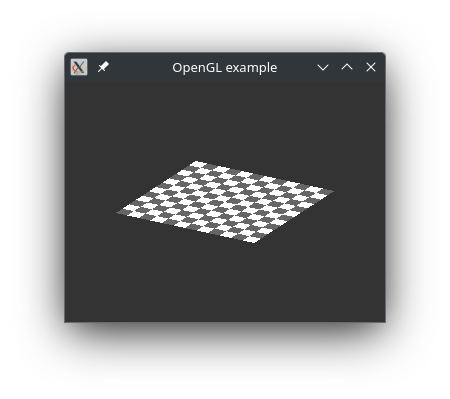
\includegraphics{rotated}}
    \end{center}
\end{slide}

\begin{slide}
    \pdfbookmark[2]{Enable Depth Testing}{depth-testing}
    \heading{3D: Enable Depth Testing}
    \begin{center}
        \begin{minipage}[c]{.8\textwidth}
            \begin{minted}[highlightlines={}]{C}
  glDepthFunc(GL_GEQUAL);
  glClipControl(GL_LOWER_LEFT, GL_ZERO_TO_ONE);
  glClearDepth(0.0);
  glEnable(GL_DEPTH_TEST);
  // ...
  while (!glfwWindowShouldClose(window)) {
    // ...
    glClear(GL_COLOR_BUFFER_BIT|GL_DEPTH_BUFFER_BIT);
    // ...
            \end{minted}
        \end{minipage}
    \end{center}
\end{slide}

\begin{slide}
    \pdfbookmark[2]{Projection Matrix}{projection}
    \heading{3D: Projection Matrix}
    \begin{center}
        \begin{minipage}[c]{.45\textwidth}
            \resizebox*{\textwidth}{!}{
\includegraphics{frustum}}
        \end{minipage}
        {\Huge $\Rightarrow$}
        \begin{minipage}[c]{.45\textwidth}
            \resizebox*{\textwidth}{!}{
\includegraphics{ndcltd}}
        \end{minipage}\vspace{-16pt}\\
        $\mathcal{P}=
         \begin{pmatrix}
            dx & 0  &  0 & 0\\
            0  & dy &  0 & 0\\
            0  & 0  &  b & a\\
            0  & 0  & -1 & 0
        \end{pmatrix}$\medskip\\
        where
        $dx=\frac{1}{\tan(\frac{1}{2}fov)}$,
        $dy=\frac{width}{height}dx$,
        $a=\frac{far\cdot near}{far-near}$,
        $b=\frac{near}{far-near}$\bigskip\\
        \url{https://www.wedesoft.de/software/2021/09/20/reversed-z-rendering/}
    \end{center}
\end{slide}

\begin{slide}
    \pdfbookmark[2]{Shader with Translation and Projection}{shader-projection}
    \heading{3D: Shader with Translation and Projection}
    \begin{center}
        \begin{minipage}[c]{.65\textwidth}
            \begin{minted}[highlightlines={4,5,11-13}]{glsl}
#version 410 core
uniform mat3 rotz;
uniform mat3 rotx;
uniform mat4 projection;
uniform float distance;
in vec3 point;
in vec2 texcoord;
out vec2 UV;
void main()
{
  vec3 translation = vec3(0, 0, -distance);
  vec3 pos = rotx * rotz * point + translation;
  gl_Position = projection * vec4(pos, 1);
  UV = texcoord;
}
            \end{minted}
        \end{minipage}
    \end{center}
\end{slide}

\begin{slide}
    \pdfbookmark[2]{Uniform Distance and Projection Matrix}{uniform-projection}
    \heading{3D: Uniform Distance and Projection Matrix}
    \begin{center}
        \begin{minipage}[c]{.95\textwidth}
            \begin{minted}[highlightlines={2,13-14}]{C}
  // ...
  glUniform1f(glGetUniformLocation(program, "distance"), 1.8);

  float fov = 45.0 * M_PI / 180;
  float near = 0.1;
  float far = 10.0;
  float dx = 1.0 / tan(0.5 * fov);
  float dy = dx * width / height;
  float a = far * near / (far - near);
  float b = near / (far - near);
  float projection[16] = {dx, 0, 0, 0, 0, dy, 0, 0,
                          0, 0, b, a, 0, 0, -1, 0};
  glUniformMatrix4fv(glGetUniformLocation(program, "projection"),
                     1, GL_TRUE, projection);
  // ...
            \end{minted}
        \end{minipage}
    \end{center}
\end{slide}

\begin{slide}
    \pdfbookmark[2]{Projected Quad}{projected-quad}
    \heading{3D: Projected Quad}
    \begin{center}
      \resizebox*{.9\textwidth}{!}{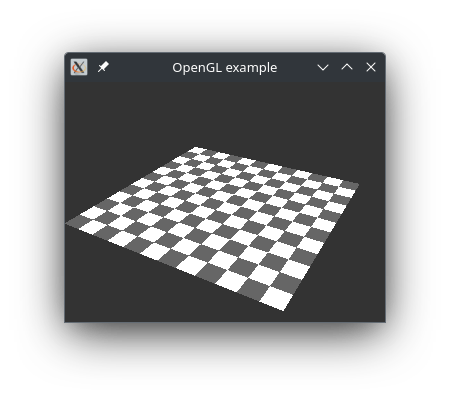
\includegraphics{projected}}
    \end{center}
\end{slide}

\begin{slide}
    \pdfbookmark[1]{Tessellation}{tessellation}
    \pdfbookmark[2]{Quad}{tessellation-quad}
    \heading{Tessellation: Quad}
    \begin{center}
        \begin{minipage}[c]{.45\textwidth}
            \resizebox*{\textwidth}{!}{
\includegraphics{original}}
        \end{minipage}
        {\Huge $\Rightarrow$}
        \begin{minipage}[c]{.45\textwidth}
            \resizebox*{\textwidth}{!}{
\includegraphics{tessellation}}
        \end{minipage}
    \end{center}
\end{slide}

\begin{slide}
  \pdfbookmark[2]{Full Pipeline}{full-pipeline}
  \heading{Tessellation: Full Pipeline}
  \begin{center}
    \resizebox*{.6\textwidth}{!}{
\includegraphics{pipeline}}
  \end{center}
\end{slide}

\begin{slide}
    \pdfbookmark[2]{Vertex Shader}{tess-vert}
    \heading{Tessellation: Vertex Shader}
    \begin{center}
        \begin{minipage}[c]{.5\textwidth}
            \begin{minted}[highlightlines={4,8}]{glsl}
#version 410 core
in vec3 point;
in vec2 texcoord;
out vec2 uv_vert;
void main()
{
  gl_Position = vec4(point, 1);
  uv_vert = texcoord;
}
            \end{minted}
        \end{minipage}
    \end{center}
\end{slide}

\begin{slide}
    \pdfbookmark[2]{Tessellation Control Shader}{tess-contr}
    \heading{Tessellation: Tessellation Control Shader}
    \begin{center}
        \begin{minipage}[c]{.95\textwidth}
            \begin{minted}[highlightlines={}]{glsl}
#version 410 core
layout(vertices = 4) out;
in vec2 uv_vert[];
out vec2 uv_contr[];
void main()
{
  if (gl_InvocationID == 0) {
    gl_TessLevelOuter[0] = 25;
    gl_TessLevelOuter[1] = 25;
    gl_TessLevelOuter[2] = 25;
    gl_TessLevelOuter[3] = 25;
    gl_TessLevelInner[0] = 25;
    gl_TessLevelInner[1] = 25;
  };
  gl_out[gl_InvocationID].gl_Position =
    gl_in[gl_InvocationID].gl_Position;
  uv_contr[gl_InvocationID] = uv_vert[gl_InvocationID];
}
            \end{minted}
        \end{minipage}
    \end{center}
\end{slide}

\begin{slide}
    \pdfbookmark[2]{Tessellation Evaluation Shader}{tess-eval}
    \heading{Tessellation: Tessellation Evaluation Shader}
    \begin{center}
        \begin{minipage}[c]{.95\textwidth}
            \begin{minted}[highlightlines={15}]{glsl}
#version 410 core
layout(quads, equal_spacing, ccw) in;
uniform mat3 rotz;
uniform mat3 rotx;
uniform mat4 projection;
uniform float distance;
in vec2 uv_contr[];
out vec2 uv_eval;
float amplitude = 0.4;
float scale = 30;
float sinc(float x)
{
  return x > 0 ? sin(x) / x : 1.0;
}
float f(vec2 v)
{
  return amplitude * sinc(scale * length(v));
}
            \end{minted}
        \end{minipage}
    \end{center}
\end{slide}

\begin{slide}
    \heading{Tessellation: Tessellation Evaluation Shader}
    \begin{center}
        \begin{minipage}[c]{.95\textwidth}
            \begin{minted}[highlightlines={9}]{glsl}
// ...
void main()
{
  vec4 pos = mix(mix(gl_in[0].gl_Position, gl_in[1].gl_Position,
                     gl_TessCoord.x),
                 mix(gl_in[3].gl_Position, gl_in[2].gl_Position,
                     gl_TessCoord.x),
                 gl_TessCoord.y);
  pos.z = f(pos.xy);
  vec3 translation = vec3(0, 0, -distance);
  gl_Position = projection *
                vec4(rotx * rotz * pos.xyz + translation, 1);
  uv_eval = mix(mix(uv_contr[0], uv_contr[1], gl_TessCoord.x),
                mix(uv_contr[3], uv_contr[2], gl_TessCoord.x),
                gl_TessCoord.y);
}
            \end{minted}
        \end{minipage}
    \end{center}
\end{slide}

\begin{slide}
    \pdfbookmark[2]{Geometry Shader}{geometry}
    \heading{Tessellation: Geometry Shader}
    \begin{center}
        \begin{minipage}[c]{.95\textwidth}
            \begin{minted}[highlightlines={10,13,16-17}]{glsl}
#version 410 core
layout(triangles) in;
in vec2 uv_eval[3];
layout(triangle_strip, max_vertices = 3) out;
out vec2 UV;
void main(void)
{
  gl_Position = gl_in[0].gl_Position;
  UV = uv_eval[0];
  EmitVertex();
  gl_Position = gl_in[1].gl_Position;
  UV = uv_eval[1];
  EmitVertex();
  gl_Position = gl_in[2].gl_Position;
  UV = uv_eval[2];
  EmitVertex();
  EndPrimitive();
}
            \end{minted}
        \end{minipage}
    \end{center}
\end{slide}

\begin{slide}
    \pdfbookmark[2]{Fragment Shader}{tess-fragment}
    \heading{Tessellation: Fragment Shader}
    \begin{center}
        \begin{minipage}[c]{.5\textwidth}
            \begin{minted}[highlightlines={}]{glsl}
#version 410 core
uniform sampler2D tex;
in vec2 UV;
out vec3 fragColor;
void main()
{
  fragColor = texture(tex, UV).rgb;
}
            \end{minted}
        \end{minipage}
    \end{center}
\end{slide}

\begin{slide}
    \pdfbookmark[2]{Compile and Link Shaders}{compile-minimal}
    \heading{Tessellation: Compile \& Link Shaders}
    \begin{center}
        \begin{minipage}[c]{\textwidth}
            \begin{minted}[highlightlines={4,9,14}]{C}
  // ...
  GLuint tessControlShader = glCreateShader(GL_TESS_CONTROL_SHADER);
  glShaderSource(tessControlShader, 1, &tessControlSource, NULL);
  glCompileShader(tessControlShader);
  handleCompileError("Tess. Control shader", tessControlShader);

  GLuint tessEvalShader = glCreateShader(GL_TESS_EVALUATION_SHADER);
  glShaderSource(tessEvalShader, 1, &tessEvalSource, NULL);
  glCompileShader(tessEvalShader);
  handleCompileError("Tess. Evaluation shader", tessEvalShader);

  GLuint geometryShader = glCreateShader(GL_GEOMETRY_SHADER);
  glShaderSource(geometryShader, 1, &geometrySource, NULL);
  glCompileShader(geometryShader);
  handleCompileError("Geometry shader", geometryShader);
  // ...
            \end{minted}
        \end{minipage}
    \end{center}
\end{slide}

\begin{slide}
    \heading{Tessellation: Compile \& Link Shaders}
    \begin{center}
        \begin{minipage}[c]{.95\textwidth}
            \begin{minted}[highlightlines={4-6}]{C}
  // ...
  GLuint program = glCreateProgram();
  glAttachShader(program, vertexShader);
  glAttachShader(program, tessControlShader);
  glAttachShader(program, tessEvalShader);
  glAttachShader(program, geometryShader);
  glAttachShader(program, fragmentShader);
  glLinkProgram(program);
  handleLinkError("Shader program", program);
  // ...
            \end{minted}
        \end{minipage}
    \end{center}
\end{slide}

\begin{slide}
    \pdfbookmark[2]{Render Patches}{render-patches}
    \heading{Tessellation: Render Patches}
    \begin{center}
        \begin{minipage}[c]{.95\textwidth}
            \begin{minted}[highlightlines={4,5}]{C}
  // ...
  while (!glfwWindowShouldClose(window)) {
    glClear(GL_COLOR_BUFFER_BIT|GL_DEPTH_BUFFER_BIT);
    glPatchParameteri(GL_PATCH_VERTICES, 4);
    glDrawElements(GL_PATCHES, 4, GL_UNSIGNED_INT, (void *)0);
    glfwSwapBuffers(window);
    glfwPollEvents();
  };
  // ...
            \end{minted}
        \end{minipage}
    \end{center}
\end{slide}

\begin{slide}
    \pdfbookmark[2]{Cleanup}{tessellation-clean-up}
    \heading{Tessellation: Cleanup}
    \begin{center}
        \begin{minipage}[c]{.7\textwidth}
            \begin{minted}[highlightlines={4-6}]{C}
  // ...
  glDeleteProgram(program);
  glDeleteShader(vertexShader);
  glDeleteShader(tessControlShader);
  glDeleteShader(tessEvalShader);
  glDeleteShader(geometryShader);
  glDeleteShader(fragmentShader);
  // ...
            \end{minted}
        \end{minipage}
    \end{center}
\end{slide}

\begin{slide}
    \pdfbookmark[2]{Result}{tess-result}
    \heading{Tessellation: Result}
    \begin{center}
      \resizebox*{.9\textwidth}{!}{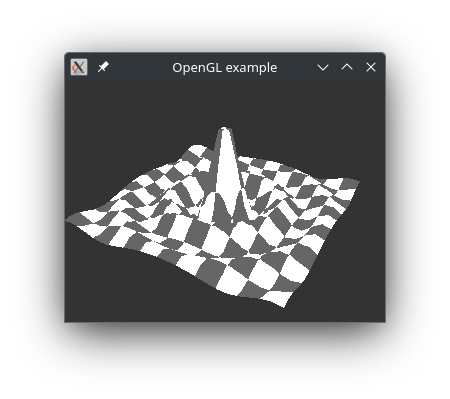
\includegraphics{sinc}}
    \end{center}
\end{slide}

\begin{slide}
    \pdfbookmark[1]{Diffuse Lighting}{diffuse}
    \pdfbookmark[2]{Tessellation Evaluation Shader}{diff-eval}
    \heading{Diffuse Lighting: Tessellation Evaluation Shader}
    \begin{center}
        \begin{minipage}[c]{.95\textwidth}
            \begin{minted}[highlightlines={16}]{glsl}
out vec3 normal_eval;
// ...
vec2 fdv(vec2 v)
{
  float l = length(v);
  if (l > 0) {
    float radial = (cos(scale * l) / (l * l) -
                    sin(scale * l) / (scale * (l * l * l)));
    return amplitude * v * radial;
  } else
    return vec2(0, 0);
}
void main()
{
  // ...
  normal_eval = rotx * rotz * vec3(-fdv(pos.xy), 1);
  // ...
}
            \end{minted}
        \end{minipage}
    \end{center}
\end{slide}

\begin{slide}
    \pdfbookmark[2]{Geometry Shader}{diff-geometry}
    \heading{Diffuse Lighting: Geometry Shader}
    \begin{center}
        \begin{minipage}[c]{.95\textwidth}
            \begin{minted}[highlightlines={2,4,8,11,14}]{glsl}
// ...
in vec3 normal_eval[3];
// ...
out vec3 normal;
void main(void)
{
  // ...
  normal = normal_eval[0];
  EmitVertex();
  // ...
  normal = normal_eval[1];
  EmitVertex();
  // ...
  normal = normal_eval[2];
  EmitVertex();
  EndPrimitive();
}
            \end{minted}
        \end{minipage}
    \end{center}
\end{slide}

\begin{slide}
    \pdfbookmark[2]{Fragment Shader}{diff-fragment}
    \heading{Diffuse Lighting: Fragment Shader}
    \begin{center}
        \begin{minipage}[c]{.85\textwidth}
            \begin{minted}[highlightlines={3,5,11}]{glsl}
#version 410 core
uniform sampler2D tex;
uniform vec3 light;
in vec2 UV;
in vec3 normal;
out vec3 fragColor;
void main()
{
  vec3 n = normalize(normal);
  float ambient = 0.2;
  float diffuse = 0.8 * max(dot(light, n), 0);
  fragColor = (ambient + diffuse) * texture(tex, UV).rgb;
}
            \end{minted}
        \end{minipage}
    \end{center}
\end{slide}

\begin{slide}
    \pdfbookmark[2]{Setup}{diff-light}
    \heading{Diffuse Lightning: Initialise Light Vector}
    \begin{center}
        \begin{minipage}[c]{\textwidth}
            \begin{minted}[highlightlines={}]{C}
  // ...
  float light[3] = {sqrt(0.5), sqrt(0.5), 0.0};
  glUniform3fv(glGetUniformLocation(program, "light"), 1, light);
  // ...
            \end{minted}
        \end{minipage}
    \end{center}
\end{slide}

\begin{slide}
    \pdfbookmark[2]{Result}{diff-result}
    \heading{Diffuse Lighting: Result}
    \begin{center}
      \resizebox*{.9\textwidth}{!}{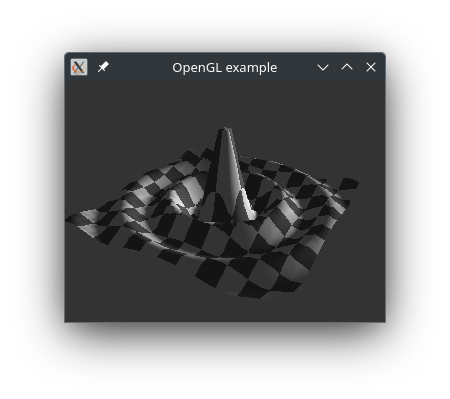
\includegraphics{diffuse}}
    \end{center}
\end{slide}

\begin{slide}
  \pdfbookmark[1]{Further Topics}{further}
  \heading{Further Topics}
  \begin{center}
    \begin{minipage}[c]{.6\textwidth}
      \begin{itemize}
        \item Face culling
        \item Phong shading
        \item Normal maps
        \item Fog
        \item Shadow mapping
        \item Volumetric rendering
        \item Physically Based Rendering (PBR)
        \item glTF asset import (e.g. using Assimp)
        \item Approaching Zero Driver Overhead (AZDO) features
        \item Compute Shaders
      \end{itemize}
    \end{minipage}
  \end{center}
\end{slide}

\begin{slide}
  \pdfbookmark[1]{References}{references}
  \pdfbookmark[2]{OpenGL Superbible}{superbible}
  \heading{References: OpenGL Superbible}
  \begin{center}
    \resizebox*{.45\textwidth}{!}{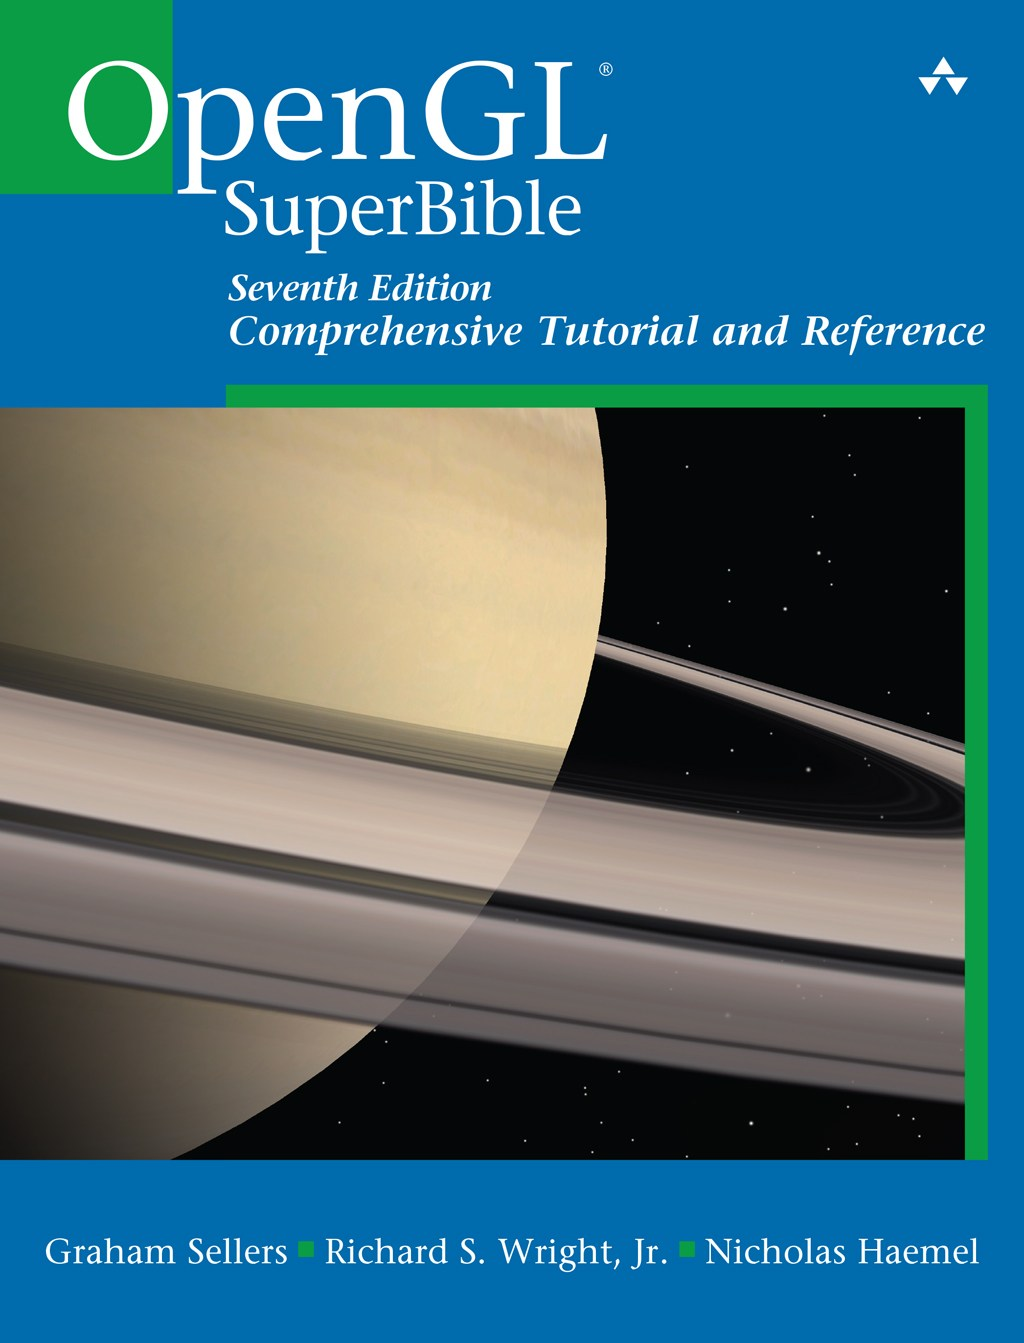
\includegraphics{superbible}}\\
    {\small \url{https://www.informit.com/store/opengl-superbible-comprehensive-tutorial-and-reference-9780134193137}}
  \end{center}
\end{slide}

\begin{slide}
  \pdfbookmark[2]{Learn OpenGL}{learnopengl}
  \heading{References: Learn OpenGL}
  \begin{center}
    \resizebox*{.45\textwidth}{!}{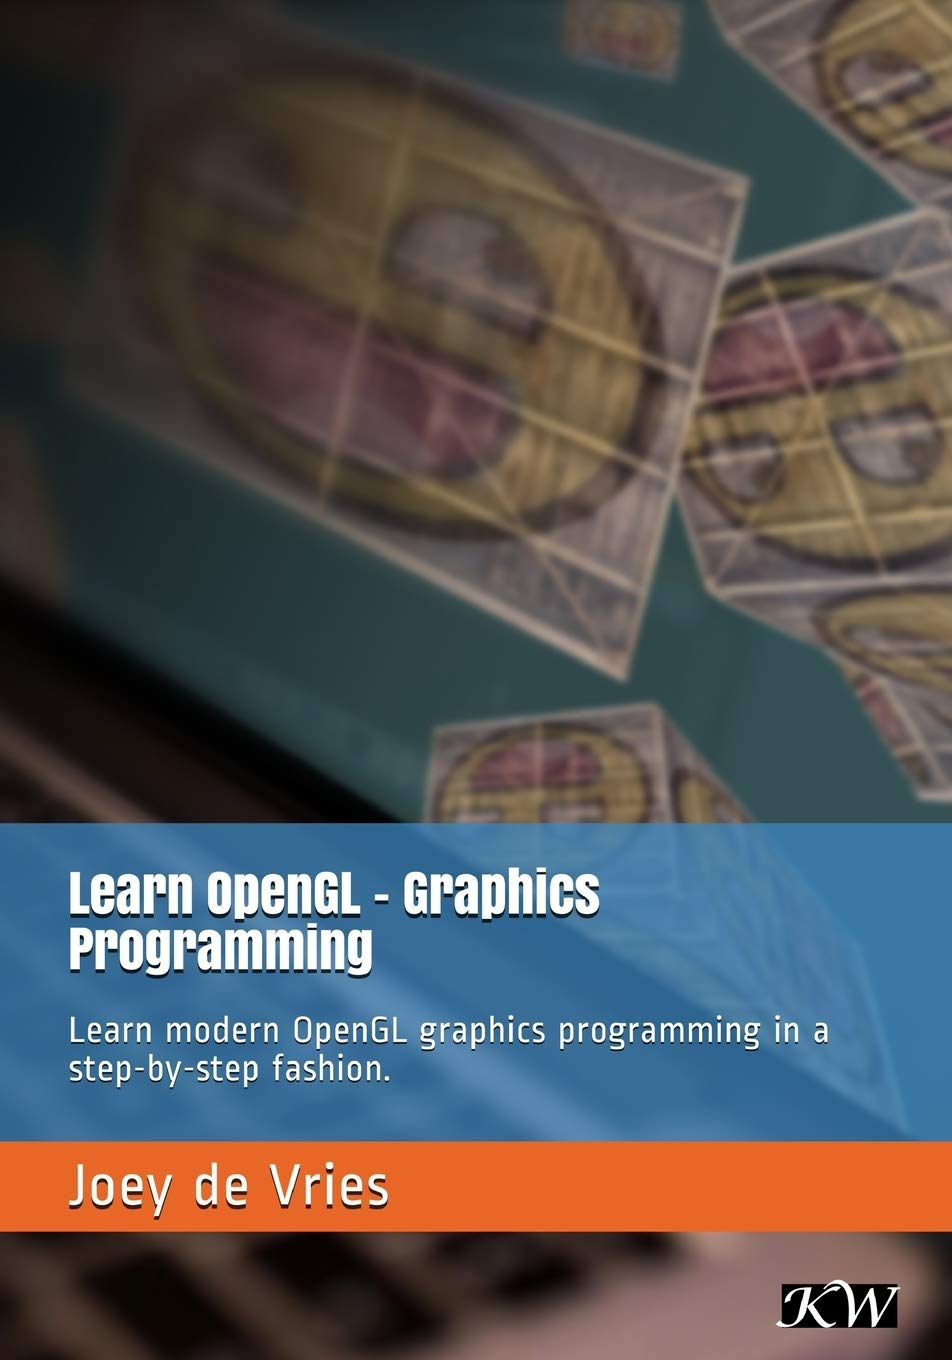
\includegraphics{learnopengl}}\\
    \url{https://learnopengl.com/}
  \end{center}
\end{slide}

\begin{slide}
  \pdfbookmark[2]{Shadertoy}{shadertoy}
  \heading{References: Shadertoy}
  \begin{center}
    \resizebox*{\textwidth}{!}{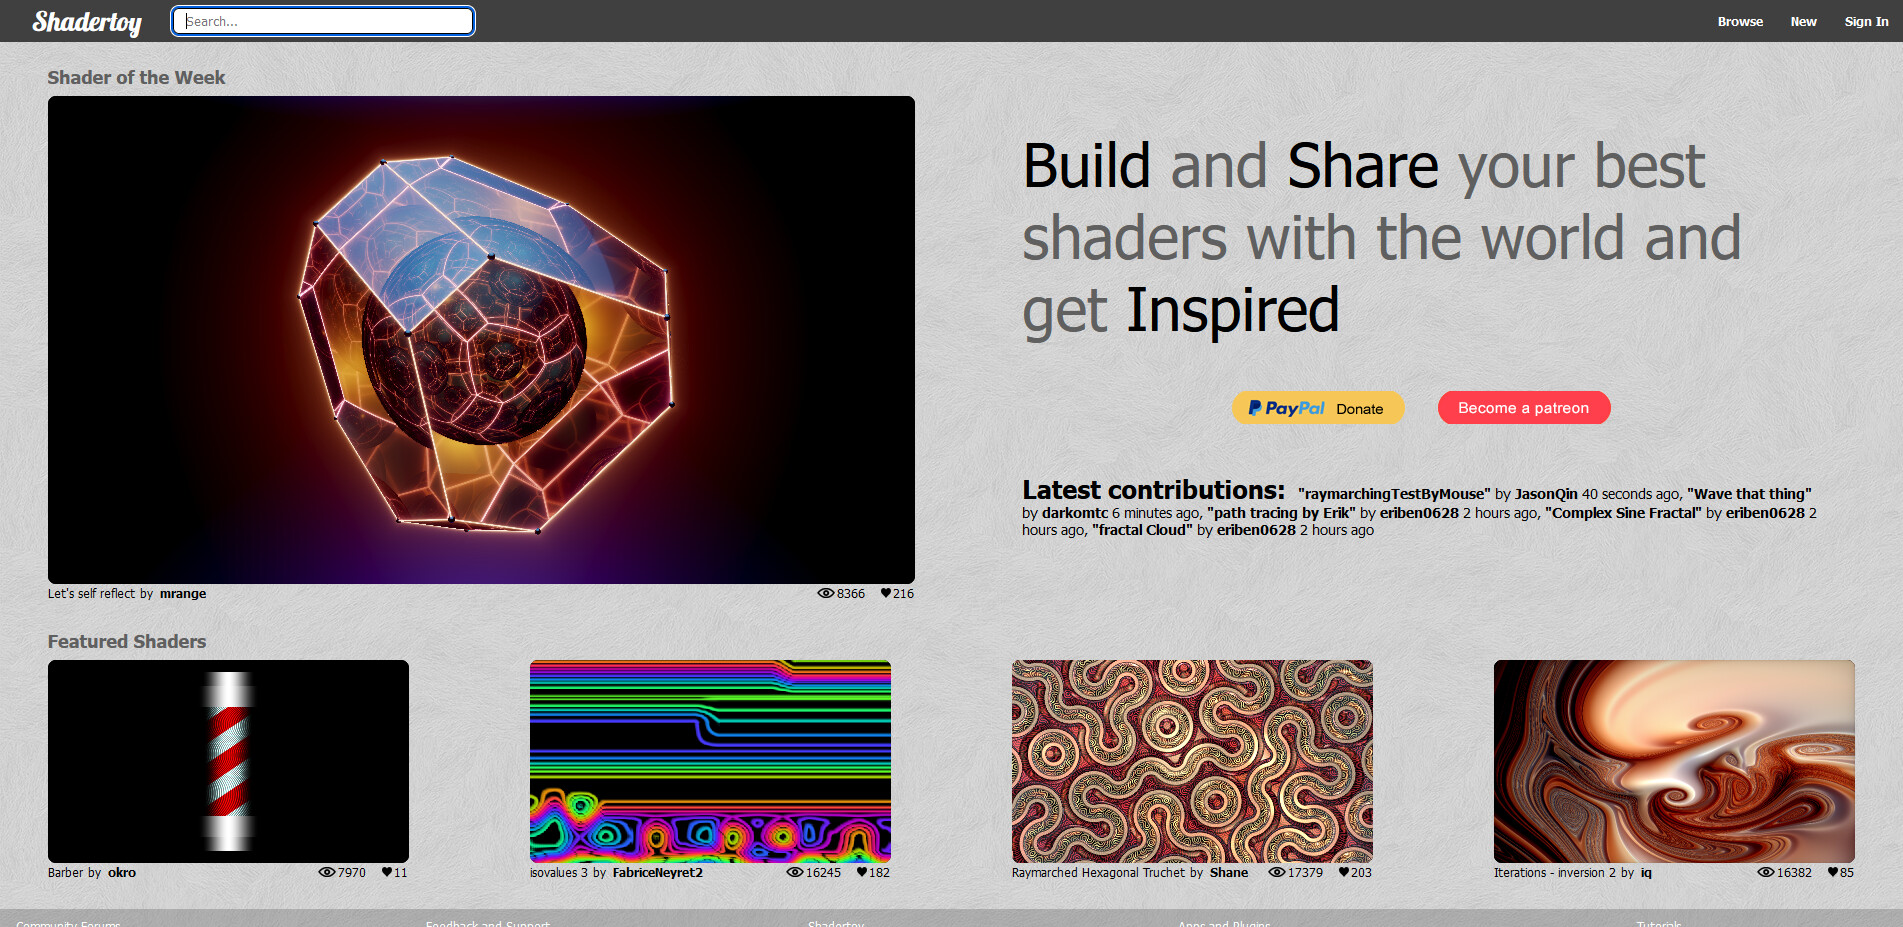
\includegraphics{shadertoy}}\\
    \url{https://www.shadertoy.com/}
  \end{center}
\end{slide}

\begin{slide}
  \pdfbookmark[1]{Questions}{questions}
  \heading{Questions?}
  \begin{center}
    \animategraphics[width=.8\textwidth,loop,autoplay]{10}{final}{1}{36}
  \end{center}
\end{slide}

\end{document}
